\documentclass[a4paper, 11pt]{article}
\usepackage[utf8]{inputenc} % Change according your file encoding
\usepackage{graphicx}
\usepackage{url}

%opening
\title{Distributed Systems, Advanced Course \\ 
		Project Report}
\author{KTH Royal Institute of Technology \\ 
	School of Information and Communication Technology \\
	Student:Fanti Machmount Al Samisti (fmas@kth.se) \\
	Student:Pradeep Perris (weherage@kth.se)}
\date{\today{}}

\begin{document}

\maketitle

\tableofcontents

\clearpage

\section{Introduction}

The project's goal was to realize a key value store in \textit{Kompics}. The most important properties are that it has to be distributed, replicated and comply to linearizable semantics. We were given many freedoms but we chose an easy and as little complicated as it can be implementation. \\
Our model is initially bootstrapped with a ,configurable yet, static set of nodes that comprise a group with a replication factor $\delta$. Each group has a segment of the key space assigned to them and a hashing function is responsible for bringing an arbitrary key value between our boundaries. \\
Finally, the data is protected from inconsistencies by employing a \textit{Read-Impose Write-Consult Majority} to bring the \textit{Atomic Register} model into our system since we can't trust our \textit{eventually perfect failure detector} so much.

\section{Design Overview}

\subsection{System Component}
The following figure depicts the overall design of the system.

{\centering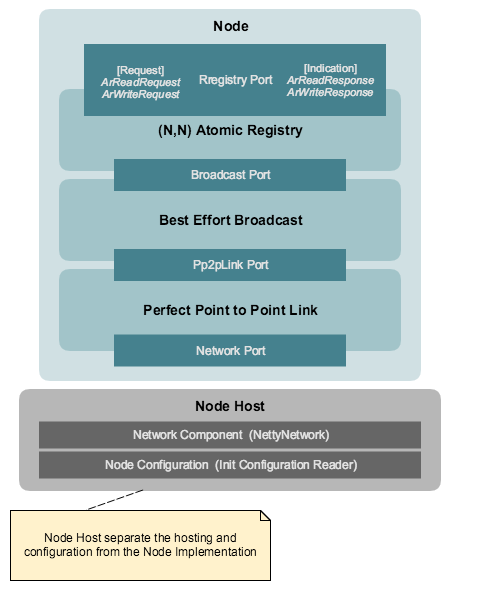
\includegraphics[scale = 0.5]{./images/design_overview.png}\par}

\subsection{Node Topology}
{\centering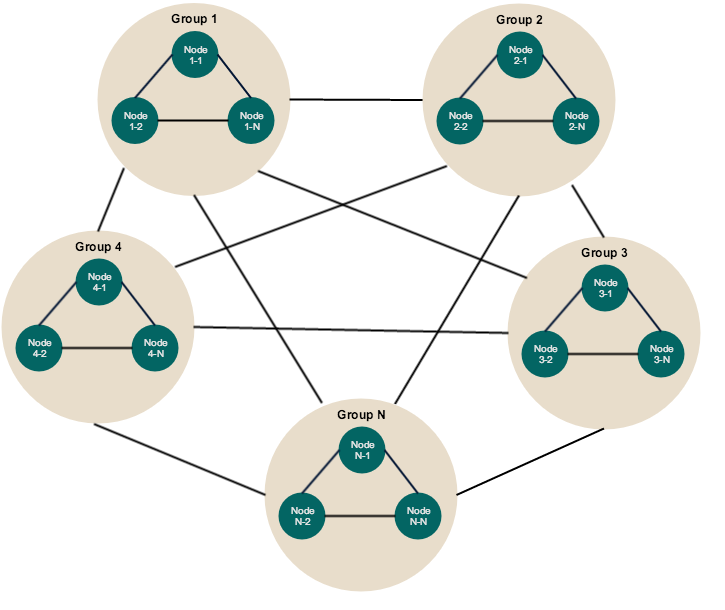
\includegraphics[scale = 0.6]{./images/node_setup.png}\par}

\section{System Abstraction and Implementation}

During our time designing and implementing the system we had a myriad of decisions to make and to motivate the `why`.

\begin{itemize}
	\item Networking protocol(TCP)
	\item Bootstrapping
	\item Group membership(Static)
	\item Failure detector($\diamond$P)
	\item Routing protocol(fully connected mesh)
	\item Replication algorithm( (N,N) Atomic Register )
\end{itemize}

\subsection{Perfect Point to Point Link}

\textit{The report should not be too long ($\approx$ 2-3 pages).}

\subsection{Best Effort Broadcast}

\textit{The report should not be too long ($\approx$ 2-3 pages).}

\subsection{(N,N) Atomic Registry}

\textit{The report should not be too long ($\approx$ 2-3 pages).}

\subsection{Failure Detector}

\textit{The report should not be too long ($\approx$ 2-3 pages).}

\subsection{Reconfiguration}
\textit{The report should not be too long ($\approx$ 2-3 pages).}

\section{System Simulations and Scenarios}

\subsection{Perfect Point to Point Link}
Perfect Point to Point Link is the base abstraction in our System Model. The properties of Perfect Point to Point Link are;
 
\begin{itemize}
	\item Reliable Delivery: If a correct process p send a message m to correct process q then q eventually delivers m.
	
	\item No Duplication: No message is delivered by a process more than once.
	
	\item No Creation: If some process q delivers a message m with sender p, then m was previously sent by process p to q.

\end{itemize}

The Reliable Delivery property is simulated in scenario \textit{Pp2pLinkScenario.java}. It let process instance of \textit{LinkPoint.java} to send a constant number of messages (1000) to another instance of \textit{LinkPoint.java}, and \textit{Pp2pSimulationObserver.java} listens on number of messages received at second instnce, and captures in a 
\textit{GlobalView}. GlobalView terminate and report to Simulation at sucessfull receival of all messages.

Although this can be even proven with the standard trasport-level protocol used in the Network model, which is TCP. 
So, As our Perfect Point to Point Link abstraction is build on top of TCP, No Duplication and No creation of messages are also satisfied.

\subsection{Best Effort Broadcast}
We have \textit{Best Effort Broadcast} component build on top of the 
Reliable Point to Point Link. That is, when the Beb Component broadcast a message, it loops through all the processes in the list and use Point to Point Send on its underlyine Pp2p Component.
The properties should be satisfied according the abstraction are:

\begin{itemize}
	
	\item Validity: If a correct process p broadcast a message m then all correct processes eventually delivers m.
		
	\item No Duplication: No message is delivered more than once.
		
	\item No Creation: If some process delivers a message m with sender p, then m was previously broadcast by process p to q.

\textit{No Duplication} and \textit{No Creation} properties are inherent from the underlyine module of 	\textit{Perfect Point to Point Link}.
\end{itemize}

The Validy property of the component is simulated and verified in \textit{BebScenario.java}. Within \textit{BebScenario.java}, it creates a constant number of (1000) of \textit{BebPointHost.java} instances as the receivers and let another instance of \textit{BebPointHost.java} to broadcast a message. \textit{BebSimulationObserver.java} simply verifies that all receviers are received the broadcast message.

Best-effort broadcast only ensures delivery amoung all correct processes, if the sender does not fail. We have the simulation [TODO] verifiy this.


\section{Conclusions}

\textit{The report should not be too long ($\approx$
  2-3 pages).}

What have you learnt from the problem presented?
Was it useful?


\end{document}
